\chapter{Neutrino Identification: Finding MicroBooNE's first Neutrinos} \label{ch:neutrinoID}
The Neutrino Identification analysis goal was to identify BNB neutrino interactions in the MicroBooNE detector collected during the first days of running. Neutrino event candidates were identified in part by using a cut on detected flash of scintillation light during the 1.6 $\micro s$ beam-spill length of the BNB as well as identifying reconstructed object from the TPC that are neutrino like. The selection performance was verified by using the 2D and 3D event displays. The selection aimed to reduce the ratio of neutrino events to cosmic-only events from the initial 1 neutrino to 675 cosmics to a ratio of 1 to 0.5 or better which is equivalent to a background reduction by a factor of 1000 or more. These selected events were used for MicroBooNE's first public displays of neutrino interactions. A clearly visible neutrino interaction with an identifiable vertex and at least 2 tracks originating from the vertex was what the analysis focused on. This analysis wasn't optimized for high purity or efficiency, but rather for very distinguishable neutrino interactions that could be shared with the public. The description of this analysis below as well as all figures come from MicroBooNE-Note-1002-Pub \cite{neutrinoid} and the corresponding internal note.
\section{Flash Finding}\label{sec:flashfinding}
Flash finding is the first step used in finding neutrino interactions. This section will detail how optical information is reconstructed as well as how analysis scripts and event filters were used.
\subsection{Flash Reconstruction}
\begin{figure}[htp!]
\centering
	\begin{subfigure}[b]{.6\textwidth}
	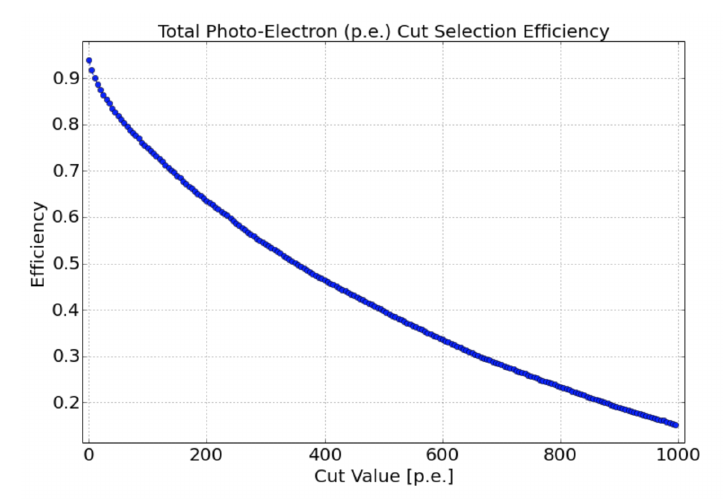
\includegraphics[width=\textwidth]{figs/totalpecut.png}
	\end{subfigure}
	\quad
	\begin{subfigure}[b]{.6\textwidth}
	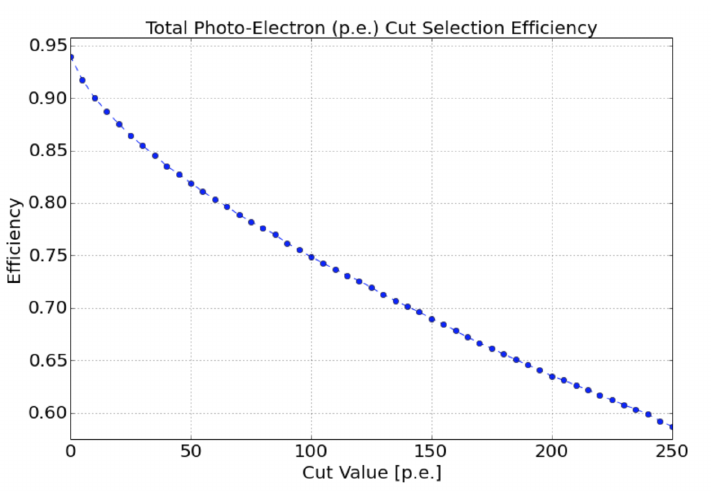
\includegraphics[width=\textwidth]{figs/totalpe_zoomed.png}
	\end{subfigure}
	\quad
\caption{Top: Efficiency for selecting beam events as a function of minimum total PE cut. Bottom: Zoomed into interesting region.}
\label{fig:PE}
\end{figure}
A definition of a flash is a collection of light above a specific photoelectron (PE) threshold seen at the same time within the detector. These signals are called optical hits. Optical hits from all the PMTs are then accumulated into 1 $\micro s$ bins of time. If a specific bin is above a set PE threshold, then the optical hits that overlap in time are then labeled as the hits from the flash. All flash reconstructed properties like average time and x/y positions are then found via the flash labeled optical hits. The total size of the flash is found by summing up the total number of photoelectrons from all PMTs. Neutrino interactions and cosmic muons will have a larger flash size compared to noise and other low-energy backgrounds, therefore a total PE cut of 50 PE was deemed sufficient and is used to reject these backgrounds in this analysis. Figure \ref{fig:PE} show the total PE versus the selection efficiency of neutrino beam events. 


\subsection{Beam Timing}
\begin{figure}[htp!]
\centering
	\begin{subfigure}[b]{.6\textwidth}
	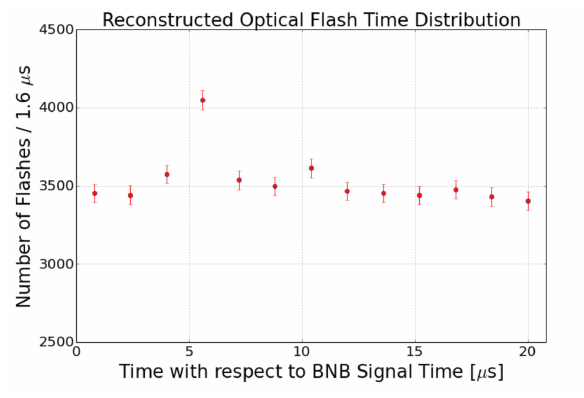
\includegraphics[width=\textwidth]{figs/flashrate_sim.png}
	\caption{Predicted distribution of flash times with respect to trigger time for 1 day of data taking at nominal rate and intensity}
	\label{fig:pe_sim}
	\end{subfigure}
	\quad
	\begin{subfigure}[b]{.6\textwidth}
	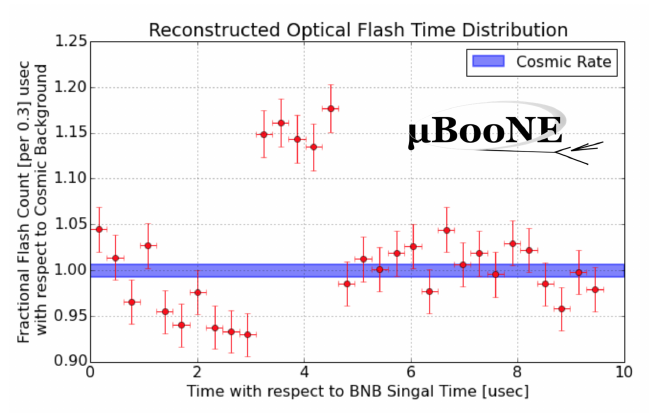
\includegraphics[width=\textwidth]{figs/flashrate.png}
	\caption{Measured distribution of flash times with a 50 PE threshold cut, with respect to trigger time. Shown as a ratio to the expected cosmic rate from off-beam data. A clear excess from neutrinos is visible between 3- 5 $\micro s$ after the trigger time. }
	\label{fig:pe_data}
	\end{subfigure}
	\quad
\label{fig:petime}
\end{figure}
It is necessary to get the specific time from flashes if one uses flashes to filter out background from neutrino interactions coincident with the neutrino beam spill period. Before a filter can be applied, an understanding of the timing of the trigger and PMT readout with respect to the arrival of neutrinos from the BNB is necessary. To do this, a 1.6 $\micro s$ window near the expected beam-time was created and verified by finding that the number of flashes was significantly above the cosmic-ray background flashes. Beam data during the first week of running, October 16th 2016 through October 22nd 2016, were used for a timing measurement. The total POT used corresponds to roughly 24 hours of data taking at nominal intensity ($4 X 10^{12} ppp$) and a 5 Hz repetition rate. Figure \ref{fig:pe_sim} shows the size of the expected neutrino signal in time using MC predictions and figure \ref{fig:pe_data} shows the neutrino signal in data. The intensity in data is lower, however a significant excess above data can still be seen.

\subsection{Event Rates}
Applying a 50 PE threshold cut inside a 1.6 $\micro s$ window reduces the cosmic-ray passing rate to 0.8\%. With a 5 Hz beam rate, this corresponds to 135 cosmics passing per hour. The neutrino passing rate for this filter is about 22 events per hour. To further increase the neutrino to cosmic ratio, TPC topology cuts were implemented and will be discussed in the following section.
\section{TPC Topology Selection}  
Two independent selection streams using TPC wire data reconstruction were implemented to further reduce cosmic event background. The first using 2D reconstructed clusters, and the second using 3D reconstructed tracks. Both streams look for neutrino interactions in the active TPC volume which are identifiable by two or more tracks originating from the same vertex.

Both 2D and 3D channels were optimized using MC simulation which used a 128 kV cathode voltage. Passing rates were calculated using a 0.8\% efficiency factor for cosmic events passing to simulate the flash finding described in section \ref{sec:flashfinding}. This efficiency factor was an overestimation and was just used to get a general feel of what signal and background rates we would actually see in data. 
\subsection{Cosmic Tagging}
The first step in TPC selection was using the geometry of cosmic tracks in an event to tag tracks that should be thrown out when searching for neutrino induced tracks. The cosmic ray muon geometry tagger runs on 3D tracks and cosmic track likeliness score to each reconstructed track. The cosmic scores are detailed below:
\begin{itemize}
\item 1: The track is tagged as entering or entering the TPC
\item 0.95: The track is a delta ray associated with a tagged track
\item 0.5: The track is either entering or exiting, but not both
\item 0.4: The track is entering or exiting through the Z boundary
\item 0: The track isn't tagged
\end{itemize}
Clusters are assigned either a 0 or 1, 1 being a cosmic. In simulation, 90\% of cosmics are tagged as cosmics and are no longer considered. Track containment affects the neutrino efficiency by 20\%. The algorithm checks that each track is contained within a boundary region of 10 cm from all sides of the TPC. This boundary region was optimized via hand-scanning of experimental data.

As can be expected, cosmic tagging is more efficient in the 3D channel (tracks) than the 2D channel (clusters) because the reconstructed tracks can use the full 3D position information of the entering and exiting points while the 2D channel mainly use the reconstructed x position of the cluster which is associated to timing. 

Cosmic tagging uses timing information to reject tracks and clusters that are outside of drift window. The drift window for 128 kV is 1.6 $\micro s$ while for 70 kV, the actual voltage MicroBooNE is running at, is 2.3 $\micro s$. Due to this variation between simulation and data, we expect to see $2.3/1.6 = 1.44$ times more cosmic induced tracks or clusters in the drift window. 
\subsection{2D Cluster Selection}
After looking at experimental cosmics data, 2D clustering performs well, while 3D track reconstruction is affected by more variations in simulation, for example noise filters. This was the motivation for having a selection only on 2D clusters in the collection (Y) plane. As stated previously, the goal of this analysis was to find identifiable neutrino interactions for use in public event displays, in future analyses, the 3D track reconstruction has been modified to further increase the tracking efficiency and has more information than just the clusters. For this analysis, however, 2D cluster information was sufficient enough for neutrino selection. 
\subsubsection{Primary Cuts}
The first cuts were used to select which clusters to consider. First the clusters must have at least ten hits on the collection plane and have a cosmic tagging score < 0.4. Only events that have at least two clusters that satisfy these primary cuts continue on.

After the initial cosmic tagging is applied, the following cuts are used to further separate identifiable neutrinos for background cosmics. 

The next cut was to remove long, vertical clusters. This was applied after seeing that most cosmic induced clusters passing were long with high angles, while neutrino induced clusters were mainly forward going. We required a good cluster to either have a projected start angle less than 30 degrees from the z axis or be less than 200 wires long. The length cut was added to make sure we don't cut any short high angle clusters that can correspond with a proton, or other highly ionizing particle associated with a long muon cluster. The 200 wire cut roughly equates to 0.6 m in the z direction, with a 3 mm wire pitch. Also, the projected angle is defined by tan $\alpha$ = $\Delta T / \Delta W$ where T is the time ticks and W is the wires. 

The last cut requires the clusters to be either 30 time ticks or 30 wires. This cut was applied to reduce small delta rays associated with a cosmic without removing proton clusters associated with a long muon cluster, which saves ideal neutrino events that have both a long minimum ionizing muon like cluster and a short highly ionizing proton like cluster.

\subsubsection{Secondary Cuts}
The secondary cuts look to match long, low-angle clusters with short, high-charge clusters. Only clusters that have passed previous cuts are used. First clusters with length greater than 100 wires are chosen, which is approximately 0.3 m in the z direction. Then we search for any cluster that is within approximately 3 cm ( 10 wires and 30 time ticks) away from the low-z end of the long cluster. This cluster must also be shorter than the first. In our reconstruction, the start and end point of a cluster can be swapped so both ends of the short cluster are compared to the long cluster. 

Now that there is a vertex match, cuts based on charge and projected opening angle are implemented. We require the short cluster to have a higher start charge than the long cluster or the long cluster be longer than 500 wires. Start charge is defined as the charge on the first wire in ADC counts. The projected opening angle must also be between 11 and 90 degrees. This last cut is intended to remove clusters that are entirely overlapping or are part of the same long track. 
\begin{table}
\begin{center}
\begin{tabular}{c c c c}
\hline
Cluster set & No Cuts & Primary Cuts & Secondary Cuts \\
\hline
Neutrinos only & 570 & 303 & 32 \\
Cosmics only ( no flash) & 308,016 & 291,879 & 602 \\
Cosmics only (w/ flash) & 2464 & 2335 & 5 \\
\hline
Neutrinos/Cosmics & 0.23 & 0.13 & 6.4 \\
\end{tabular}
\caption{Passing rates for 2D cluster cuts for neutrino on MC set and a cosmic only MC set. First column shows event rates with no cuts applied to both sets. Columns two and three show event rates after primary and secondary cuts are applied. Line three shows the second line scaled with the flash finding factor of 0.008. All events are normalized to per day assuming we are running at 5 Hz.}
\label{table:eventrate}
\end{center}
\end{table}
The resulting neutrino/cosmic event rate per day is shown in table \ref{table:eventrate}. Figures \ref{fig:2dprimarycut} and \ref{fig:2dsecondarycuts} shows the percentages of clusters that pass each primary and secondary cuts.     

\begin{figure}[htp!]
\centering
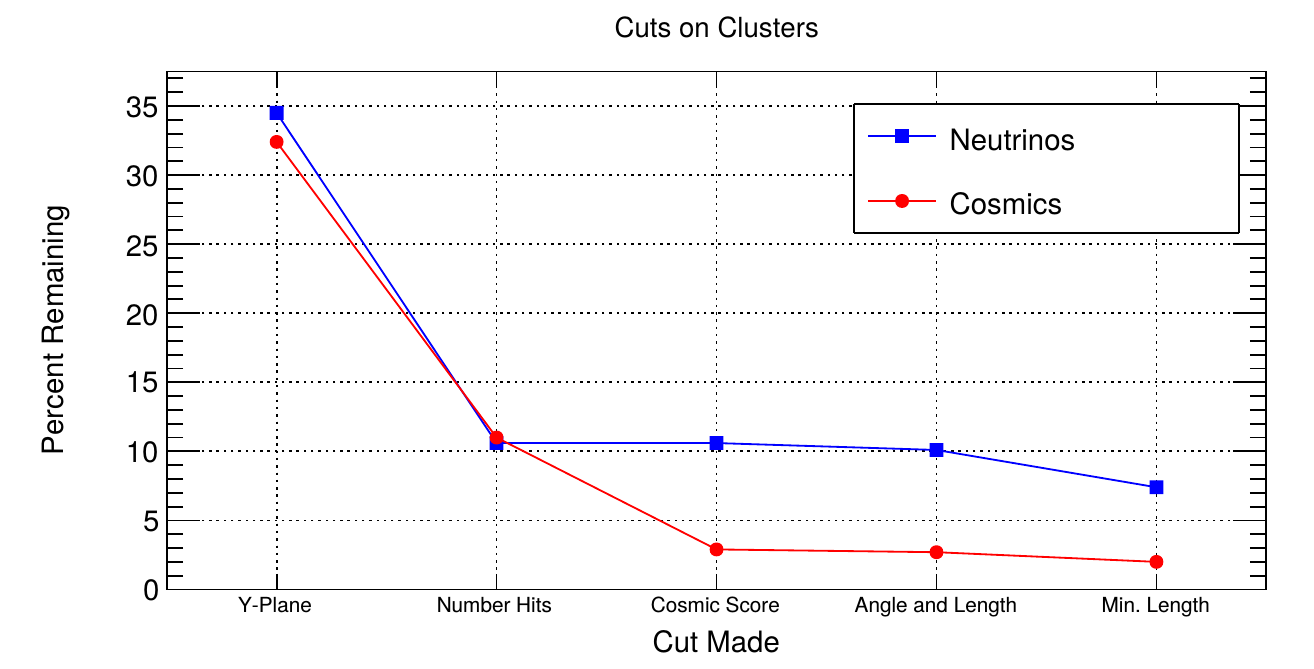
\includegraphics[width=\textwidth]{figs/2dprimarycut.png}
\caption{Percent of good clusters remaining for neutrinos and cosmics after the primary cuts were applied. This is relative to total number of initial clusters.}
\label{fig:2dprimarycut}
\end{figure}

\begin{figure}[htp!]
\centering
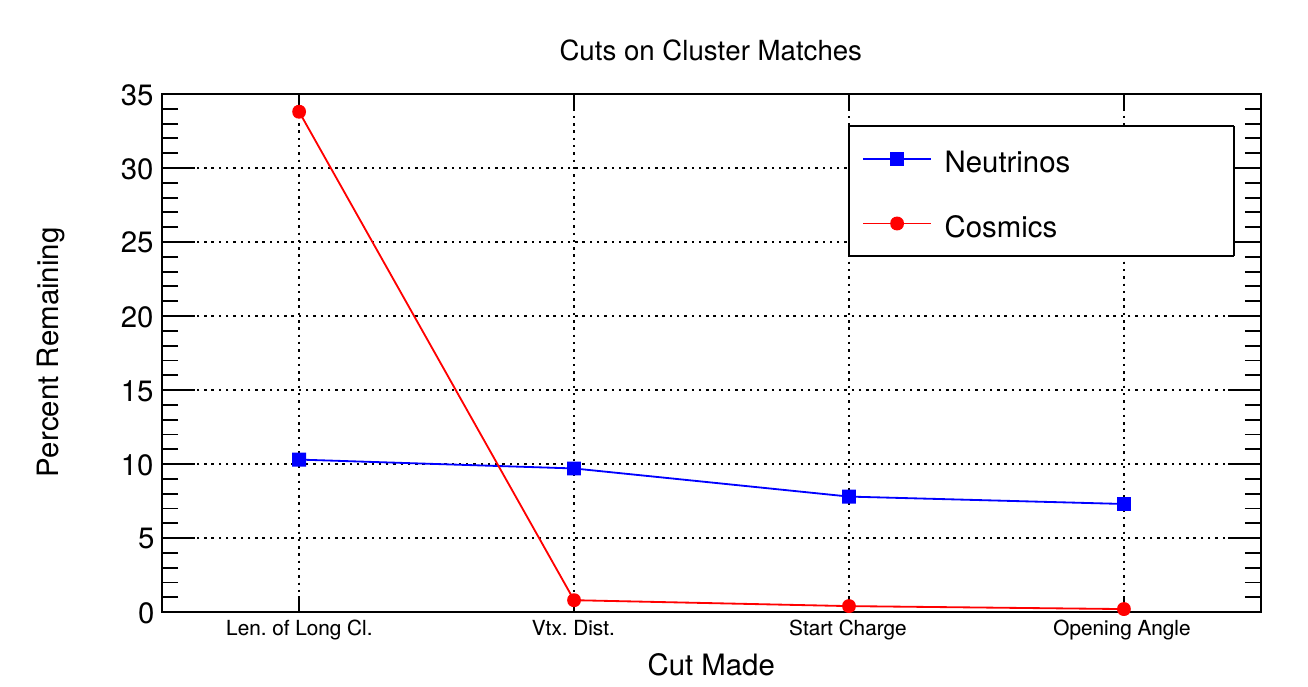
\includegraphics[width=\textwidth]{figs/2dsecondarycut.png}
\caption{Percent matched cluster pairs remaining for neutrinos and cosmics after secondary cuts applied. This is relative to the number of events that contain clusters which pass the primary cuts.}
\label{fig:2dsecondarycuts}
\end{figure}

\subsection{3D Tracks and vertices Selection}
The neutrino selection for the 3D channel was based on a reconstructed vertex and two tracks. All vertices and tracks were looped over that had a cosmic tag score < 0.4 and the distances below were calculated:
\begin{itemize}
\item d: distance between the start points of the two tracks.
\item $d_1$: distance between vertex and start of track 1.
\item $d_2$: distance between vertex and start of track 2.
\end{itemize}
The maximum distance of all three is then selected as the important characteristic per trio. The best trio is the one that has the smallest maximum distance. The $min(max_{d})$ for all trios in an event were plotted for BNB neutrino events and for cosmics to find the best cut value for each tracking algorithm. The distribution of $min(max_{d,i})$ is smaller for neutrinos than for cosmics. The cut values for different tracking and clustering algorithms are shown below. These cut values were chosen to minimize the cosmic background to 20\%. 
\begin{itemize}
\item trackkalmanhit with cccluster $min(max_{d,i})$ < 3 cm.
\item trackkalmanhit with pandoraNu $min(max_{d,i})$ < 4.5 cm.
\item pandoraNu with cccluster $min(max_{d,i})$ < 5 cm.
\end{itemize}

\subsection{TPC Updates}
After doing a visual hand-scanning of the first beam data processed with the filters detailed above, the events passing had a larger contamination of background than expected. This was mainly due to the reconstruction performing better on simulation than on data. Due to this, additional cuts on both streams needed to be implemented in order to increase signal/background ratio. These cuts were added on top of the filters described above and further reduce the event count. 
\subsubsection{2D Filter Updates}
The main background observed in the 2D filter were Michel events, where the muon and electron formed two connected clusters. These events were rejected by comparing the start and end charge deposition of the long cluster (i.e muon particle). The start charge deposition must be less than the end charge deposition. This cut is implemented because muons have a higher ionization loss at the end. 
\subsubsection{3D Filter Updates}
It was seen that cosmic tracks can often originate or end at the same point, therefore faking a signal. Cosmic tracks, however, are mostly vertical. By requiring the angle of the longer track have a cosine greater than 0.85 with respect to the z-axis as well as requiring the longer track to have a length greater than 10 cm, we can reduce this background. 
\section{Conclusion}
After processing these filters in parallel, it was shown that the 3D filter had a higher purity than the 2D filter because of the higher cosmic rejection being used due to 3D reconstruction. The 2D filter is blind to track entering/exiting from the top or bottom of the TPC. Although the 3D filter had a higher purity, the 2D filter was still able to find identifiable events in data that were used as public event displays. A sample of event displays are shown in figures \ref{fig:2dimage} and \ref{fig:3dimage}.

\begin{figure}[htp!]
\centering
	\begin{subfigure}[b]{.8\textwidth}
	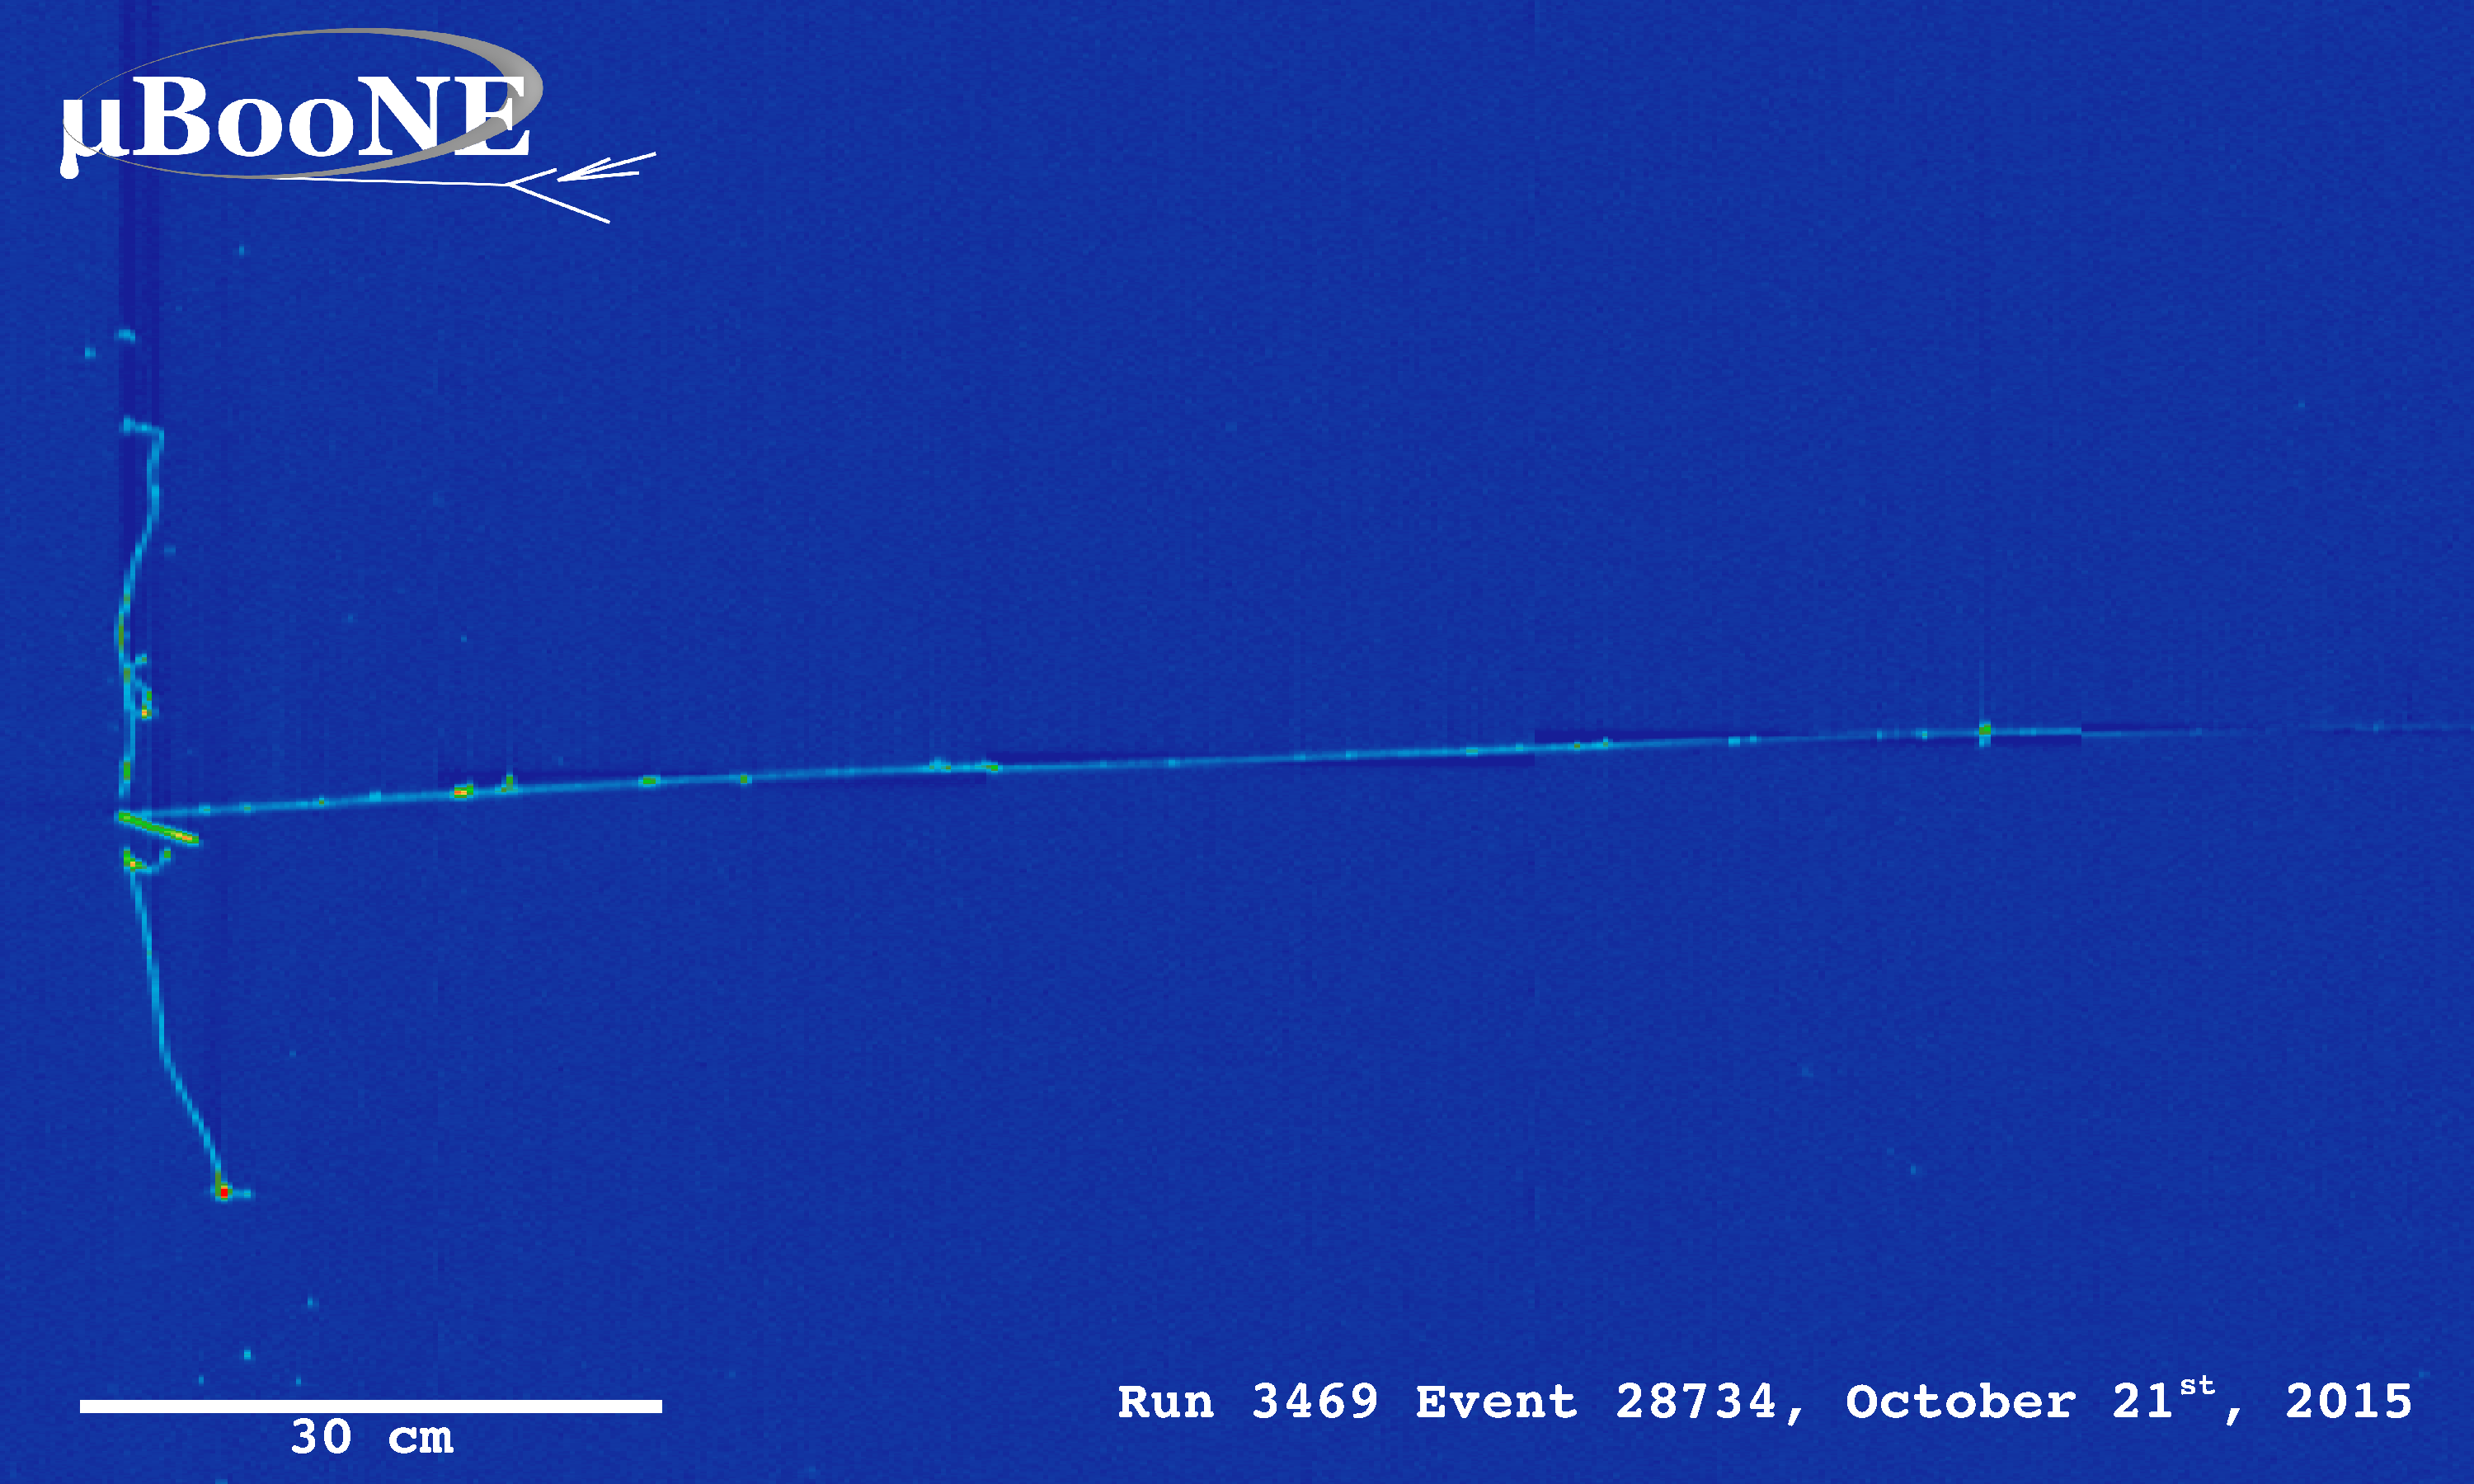
\includegraphics[width=\textwidth]{figs/first_neutrino_pdfs/run3469_subrun574_event28734_col.pdf}
	\end{subfigure}
	\quad
	\begin{subfigure}[b]{.8\textwidth}
	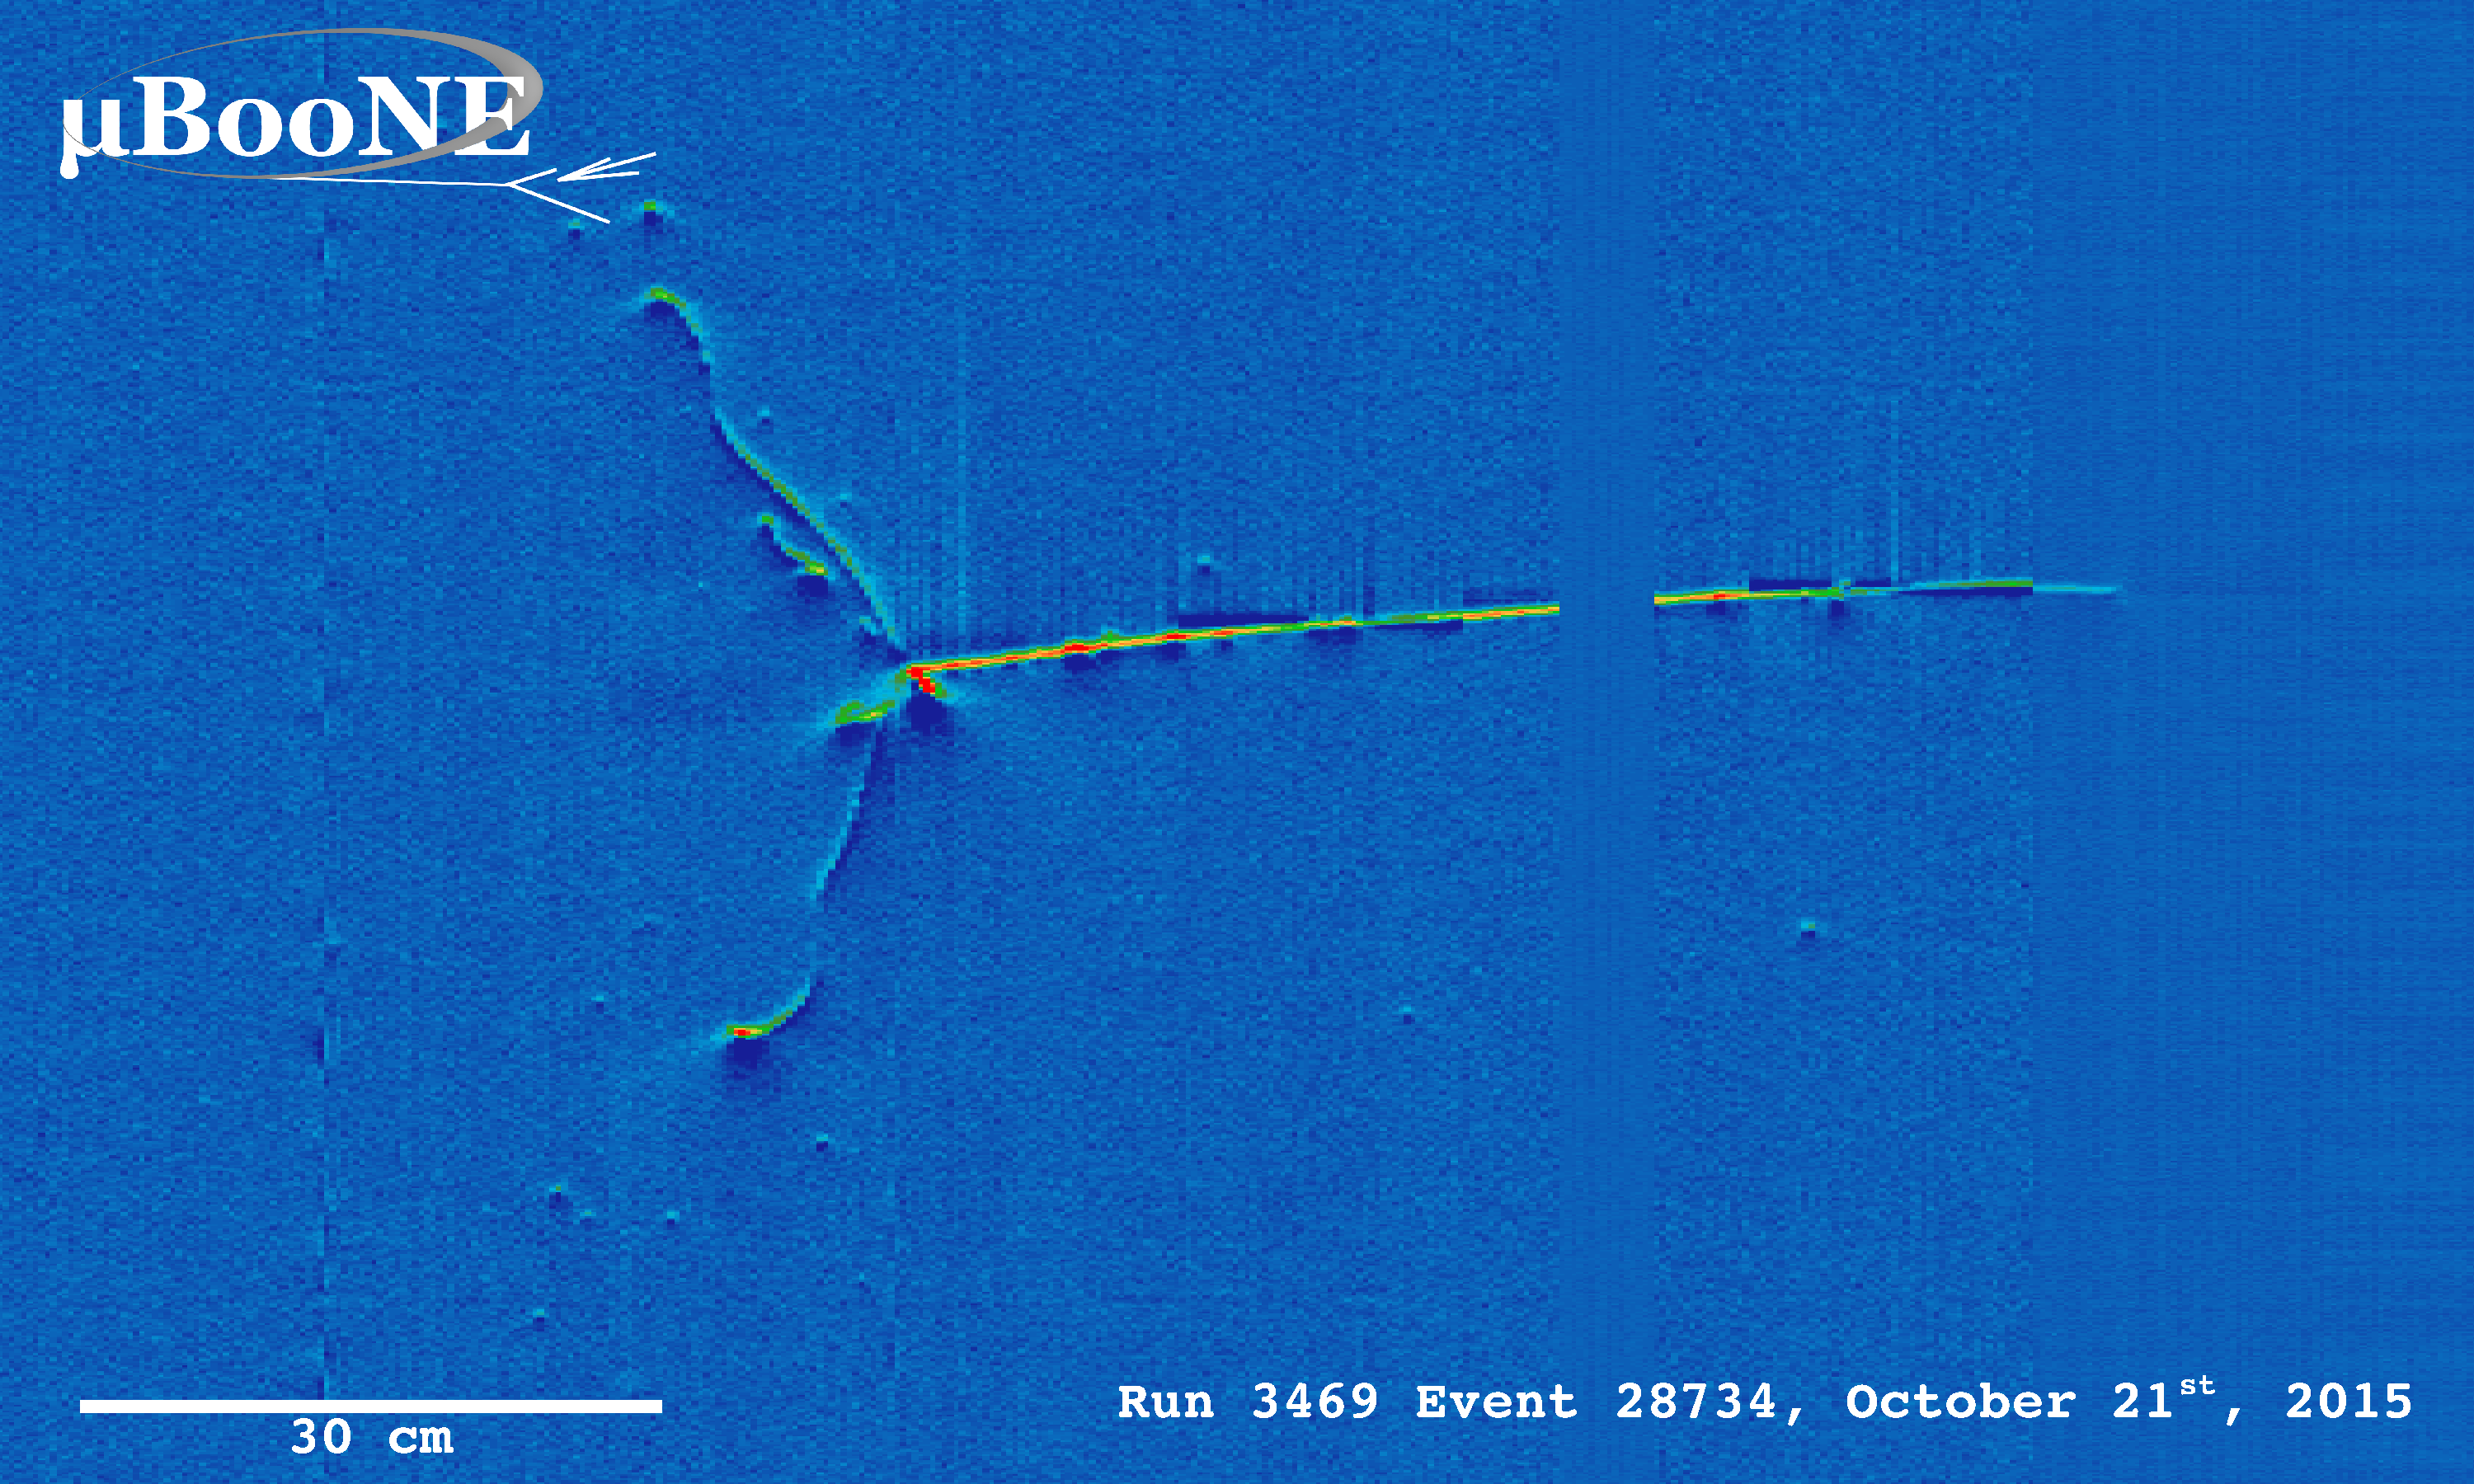
\includegraphics[width=\textwidth]{figs/first_neutrino_pdfs/run3469_subrun574_event28734_ind0.pdf}
	\end{subfigure}
	\quad
	\begin{subfigure}[b]{.8\textwidth}
	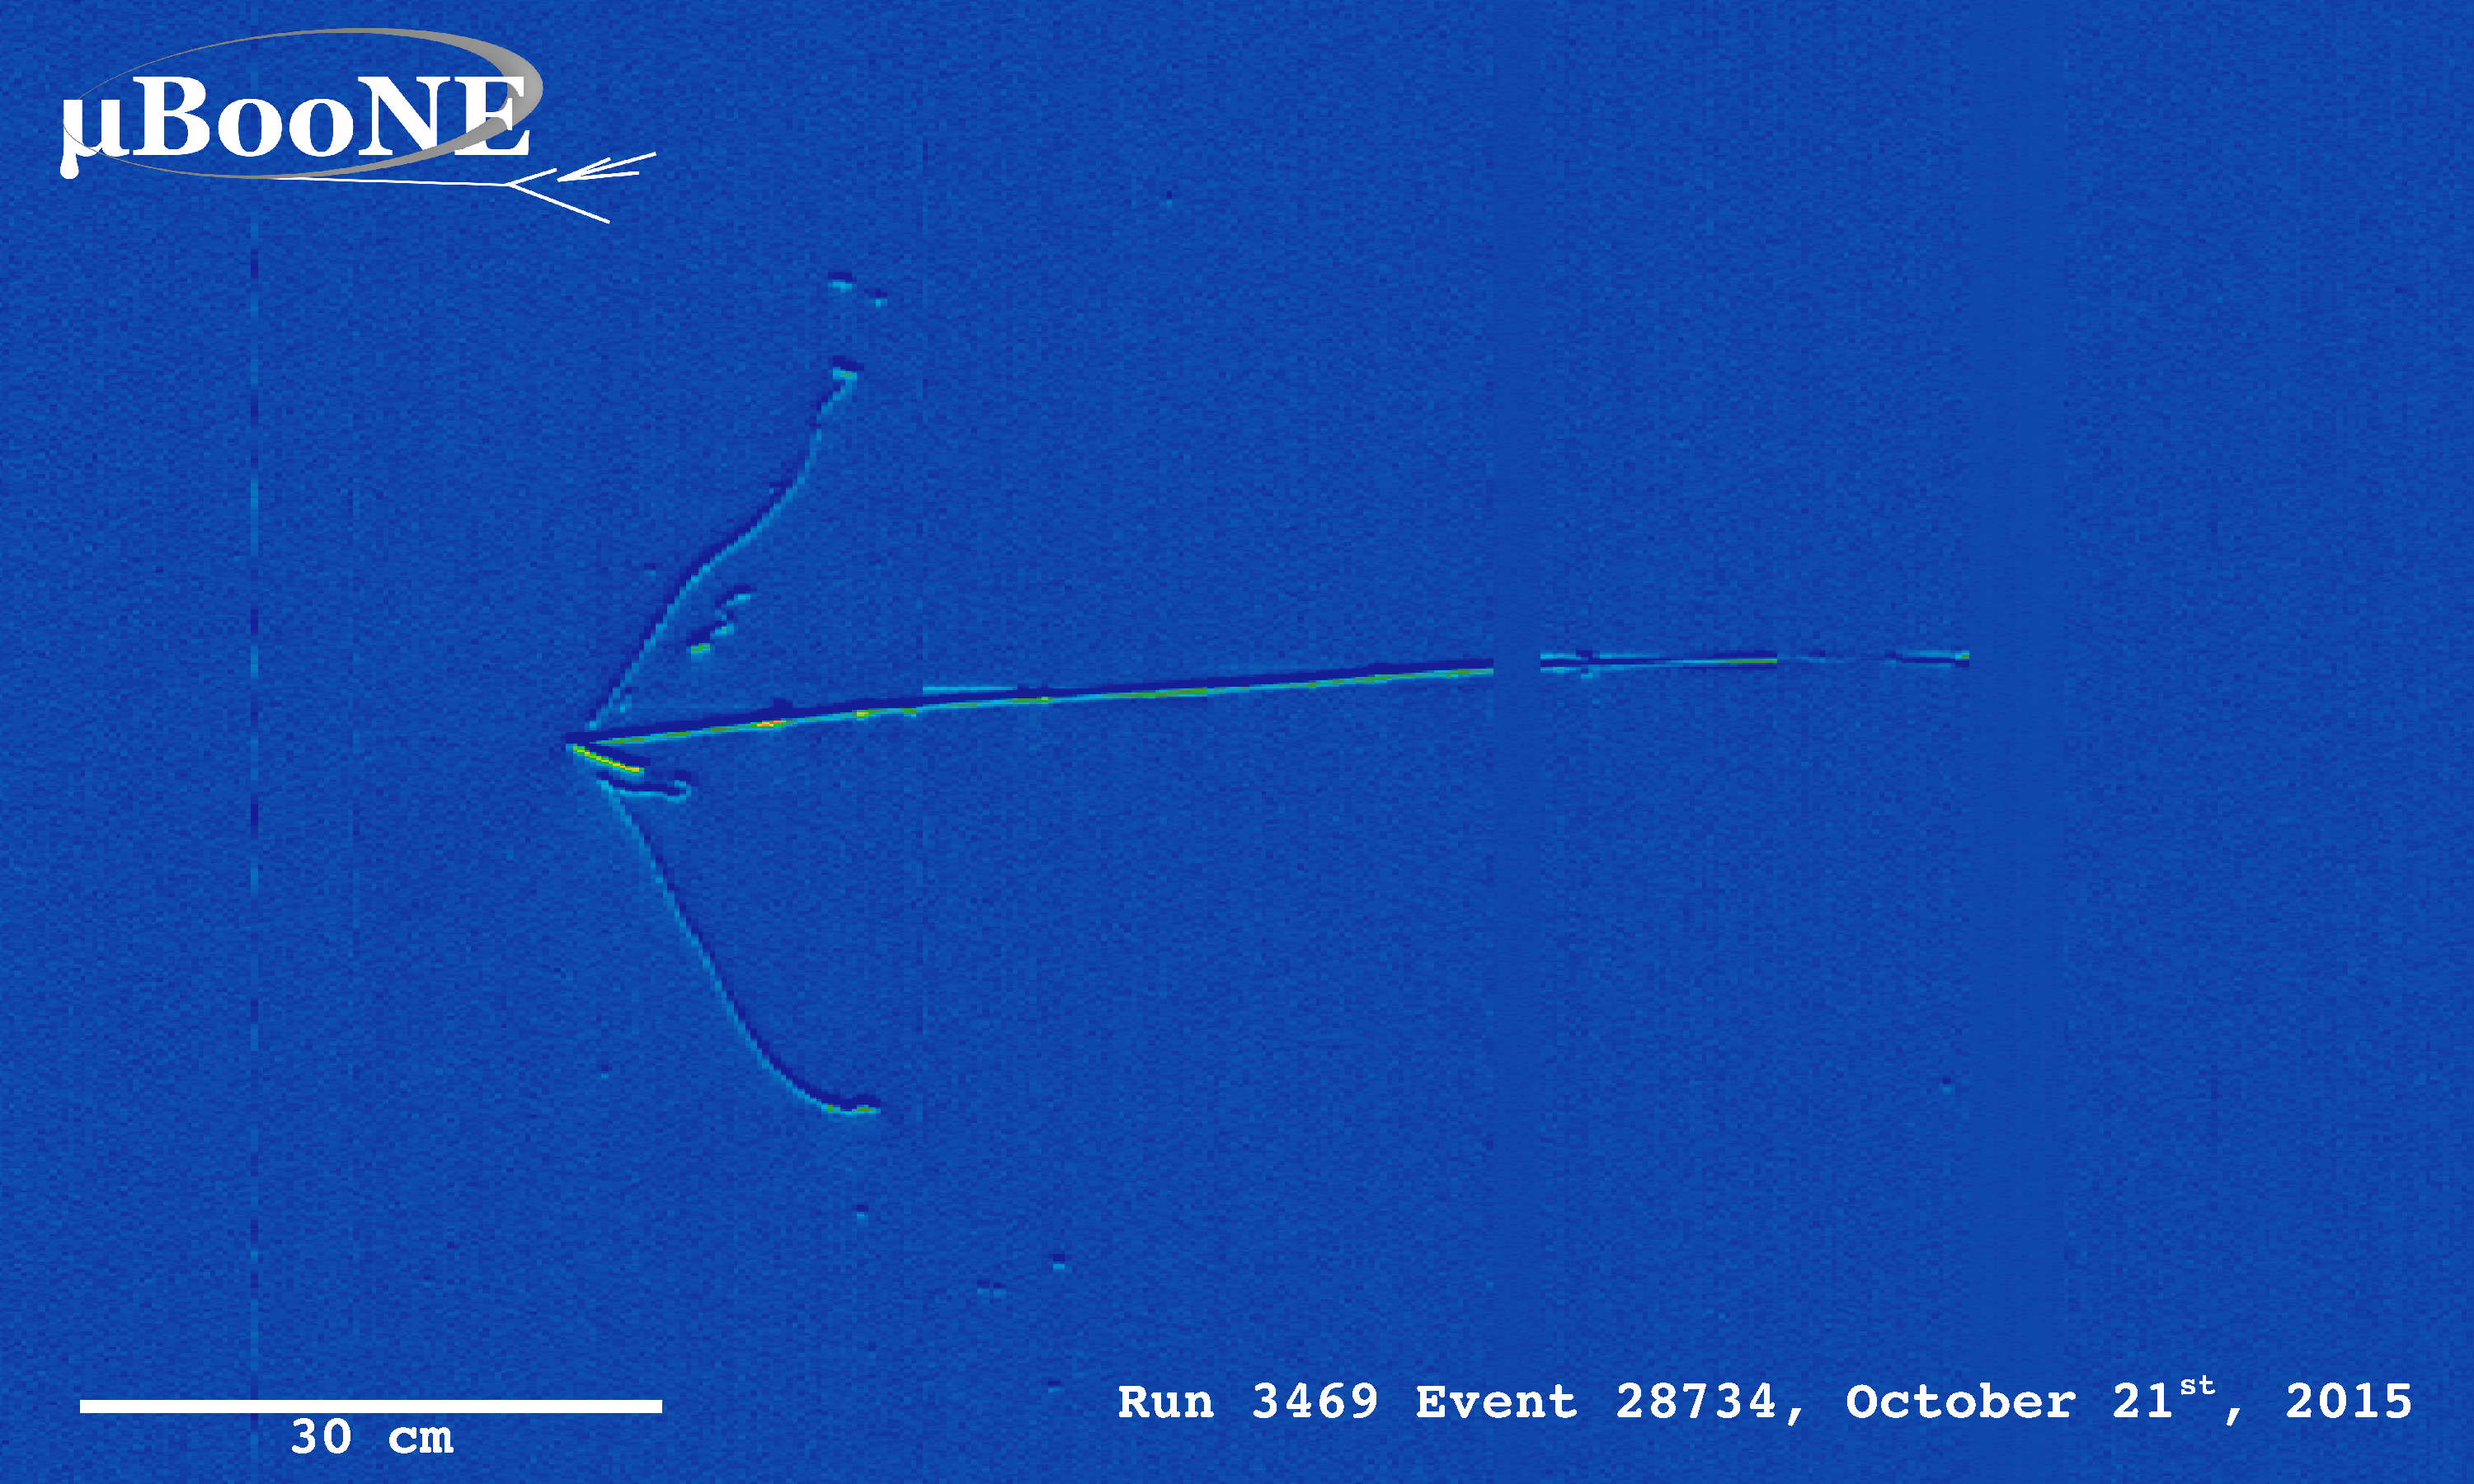
\includegraphics[width=\textwidth]{figs/first_neutrino_pdfs/run3469_subrun574_event28734_ind1.pdf}
	\end{subfigure}
	\quad
\caption{First Neutrino Interaction Candidate Events from MicroBooNE}
\label{fig:2dimage}
\end{figure}

\begin{figure}[htp!]
\centering
	\begin{subfigure}[b]{.8\textwidth}
	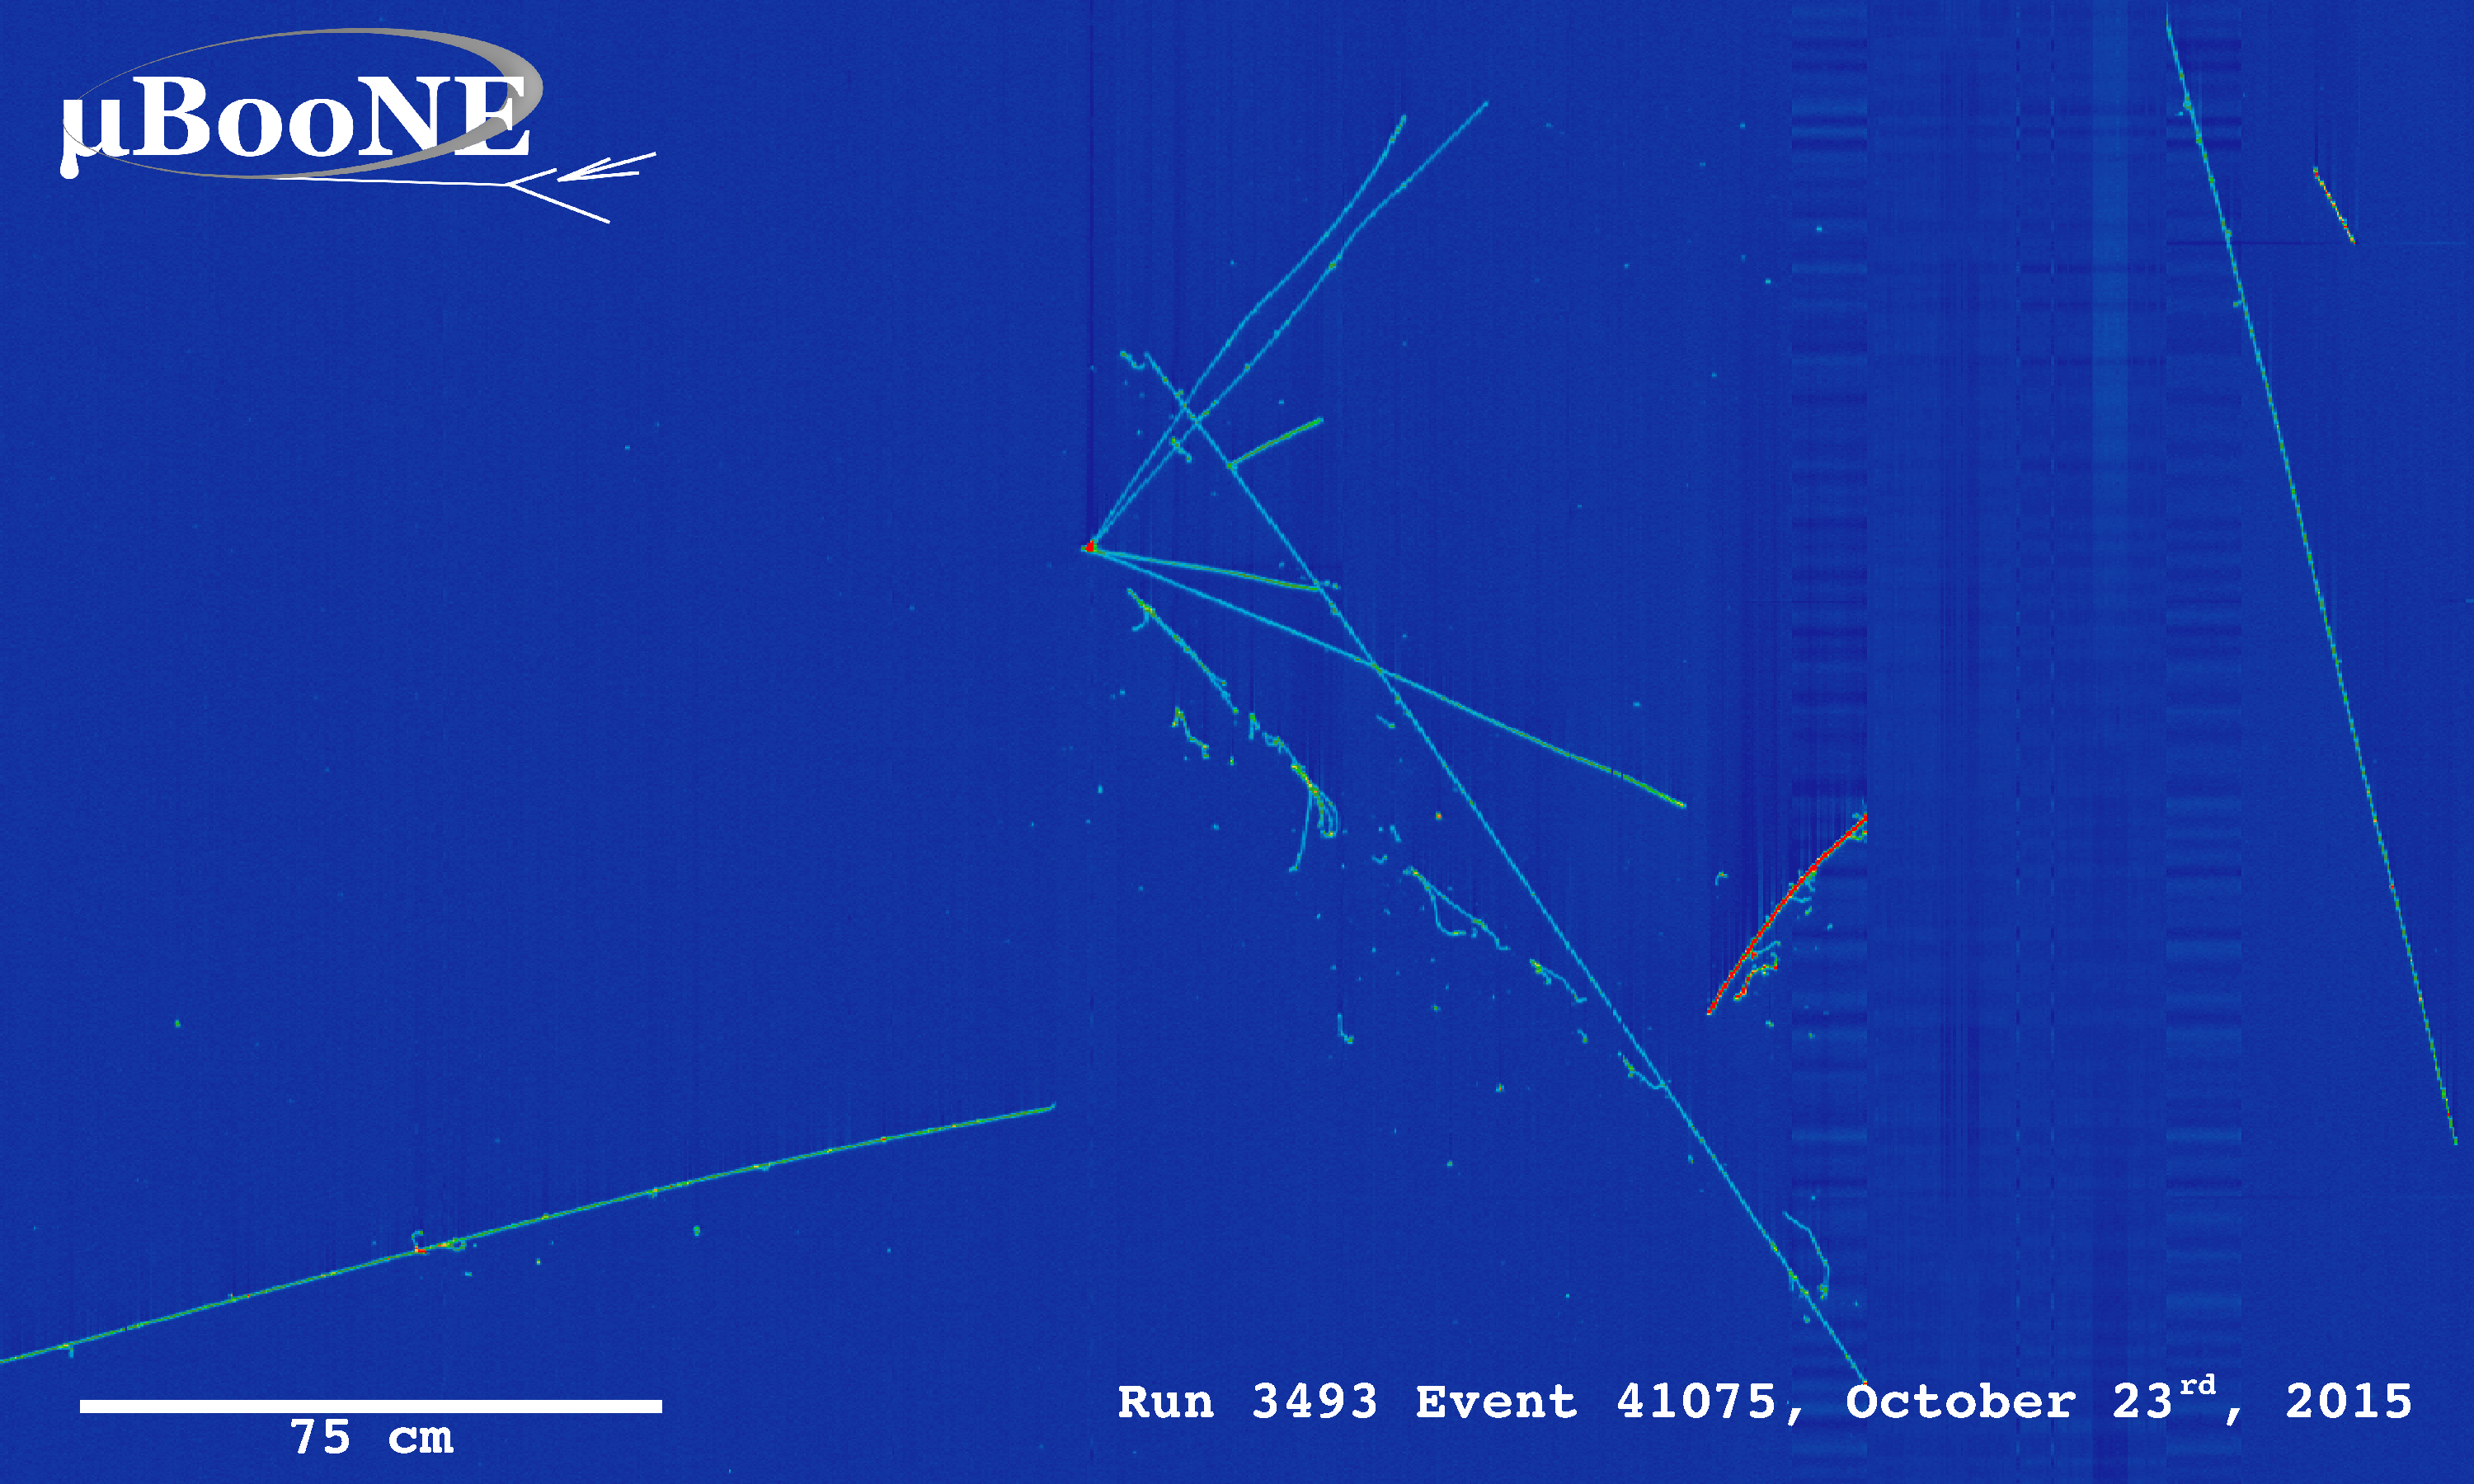
\includegraphics[width=\textwidth]{figs/first_neutrino_pdfs/run3493_subrun821_event41075_col.pdf}
	\end{subfigure}
	\quad
	\begin{subfigure}[b]{.8\textwidth}
	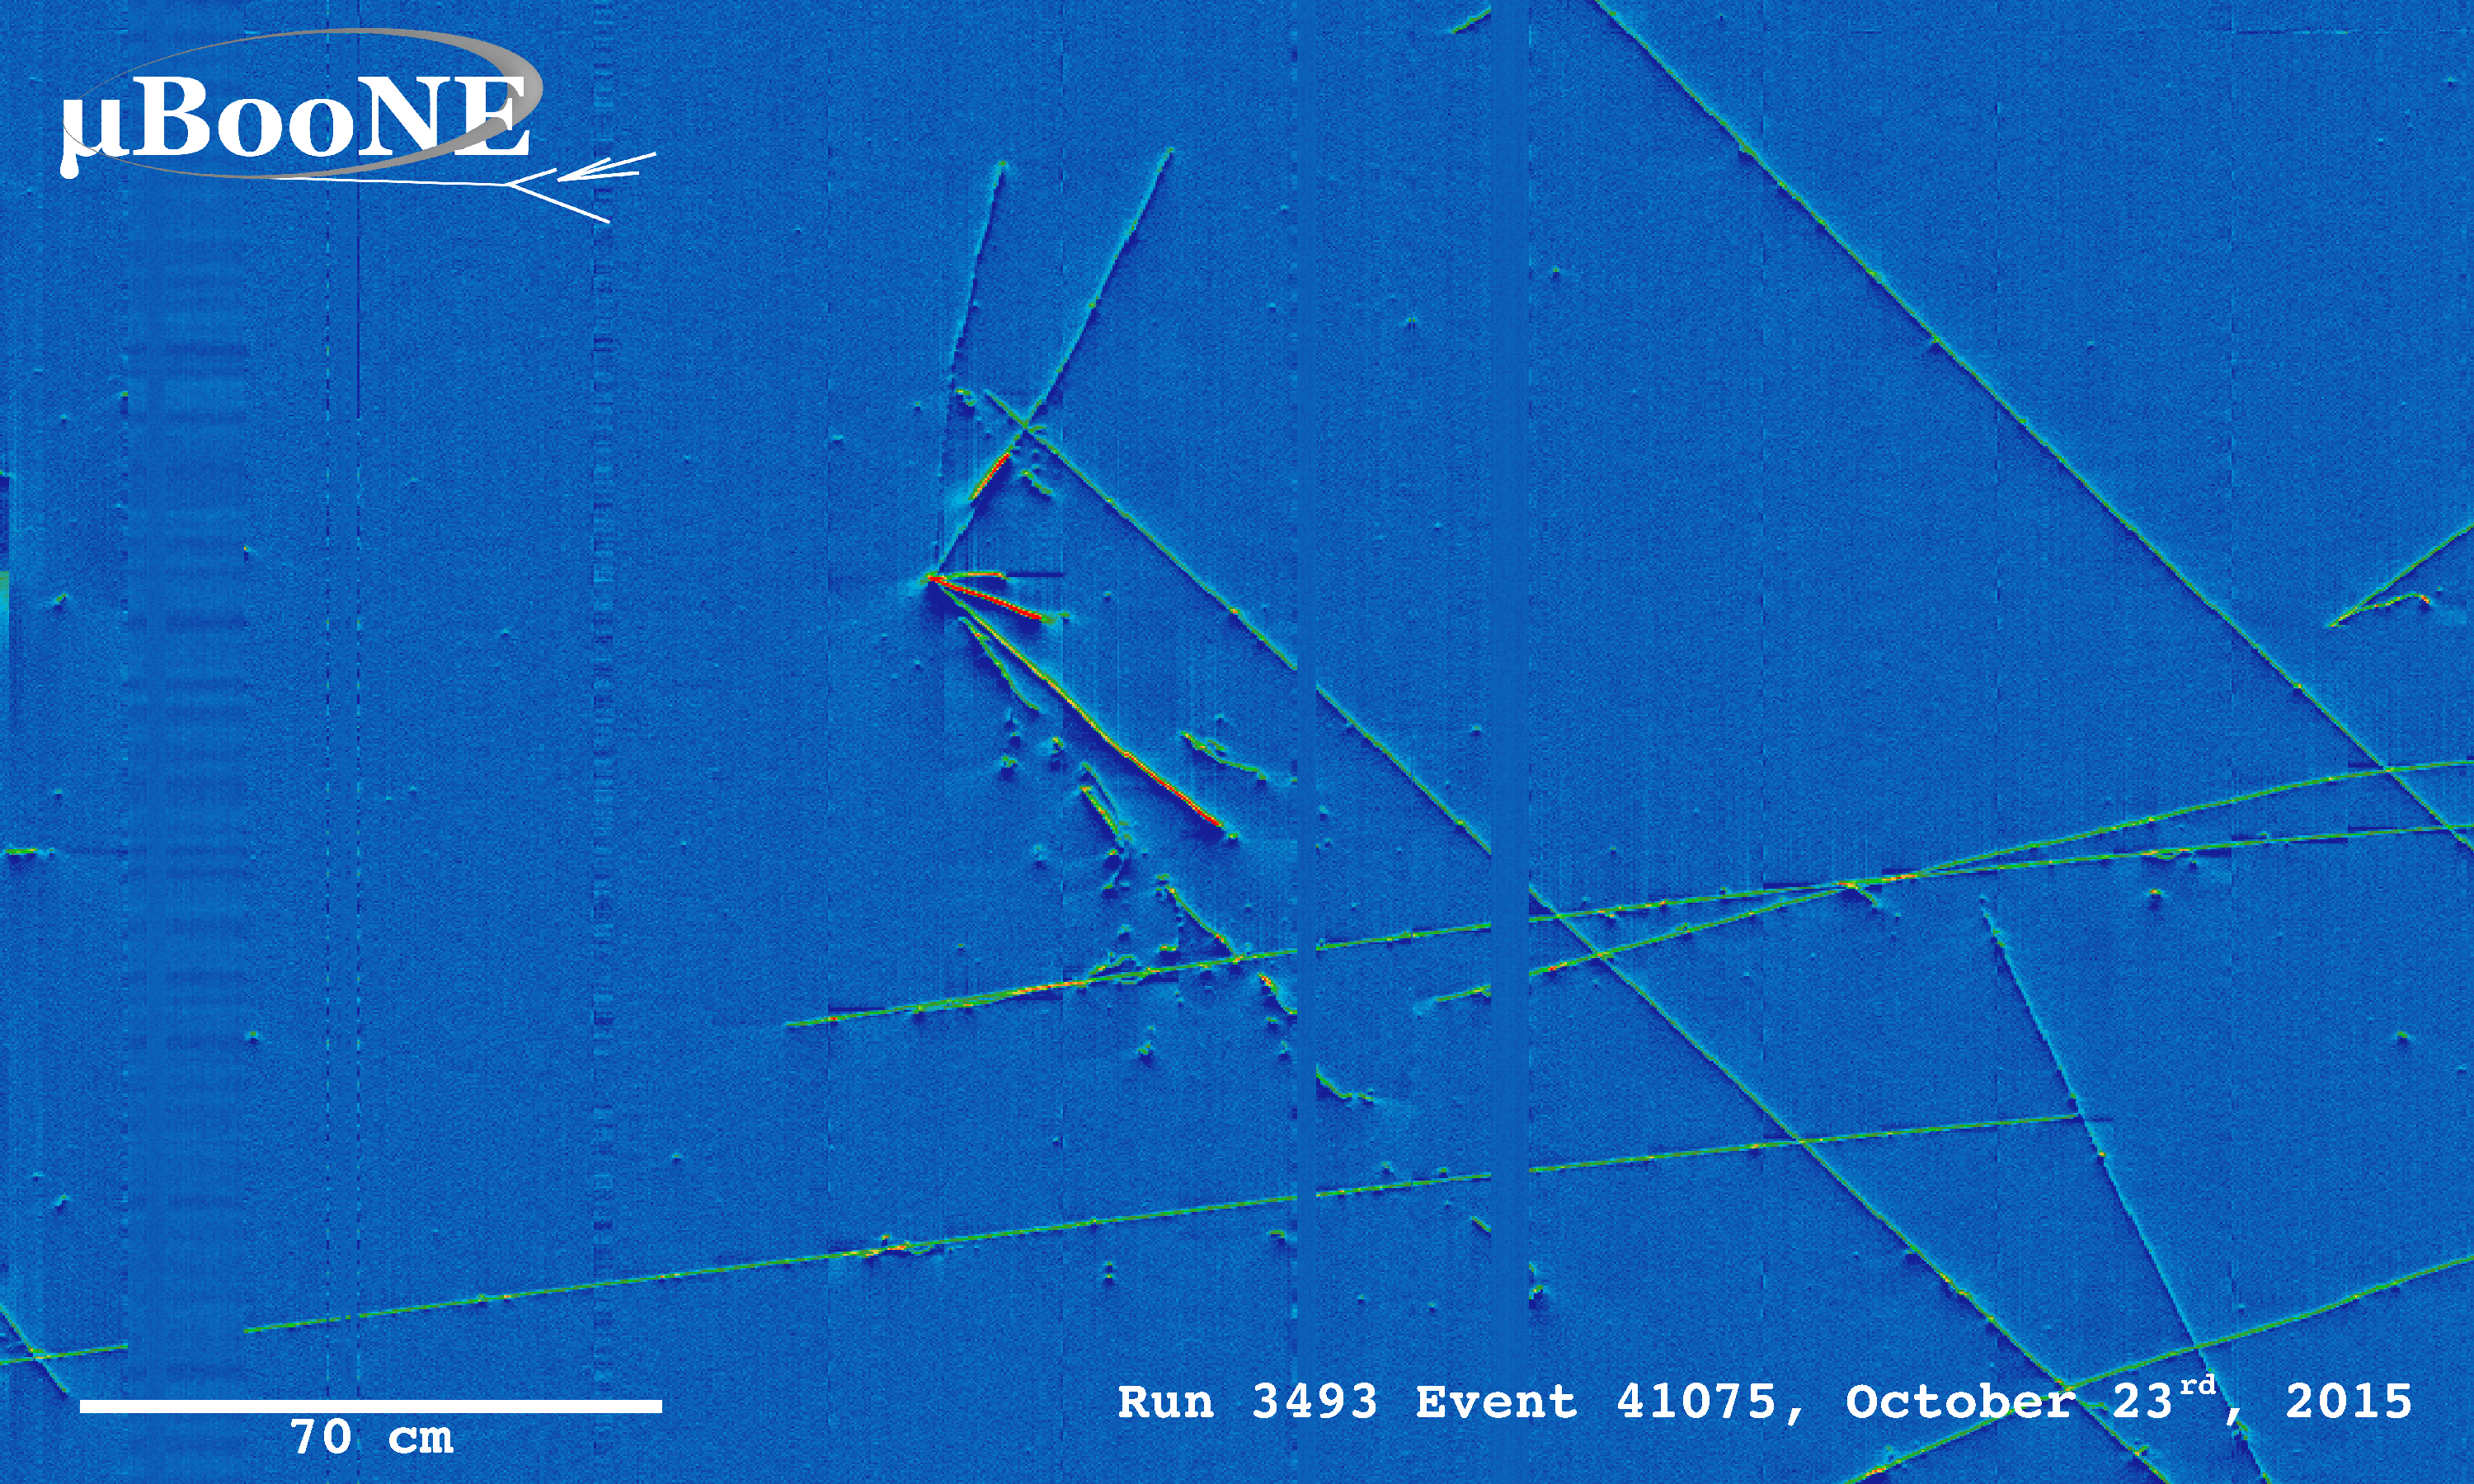
\includegraphics[width=\textwidth]{figs/first_neutrino_pdfs/run3493_subrun821_event41075_ind0.pdf}
	\end{subfigure}
	\quad
	\begin{subfigure}[b]{.8\textwidth}
	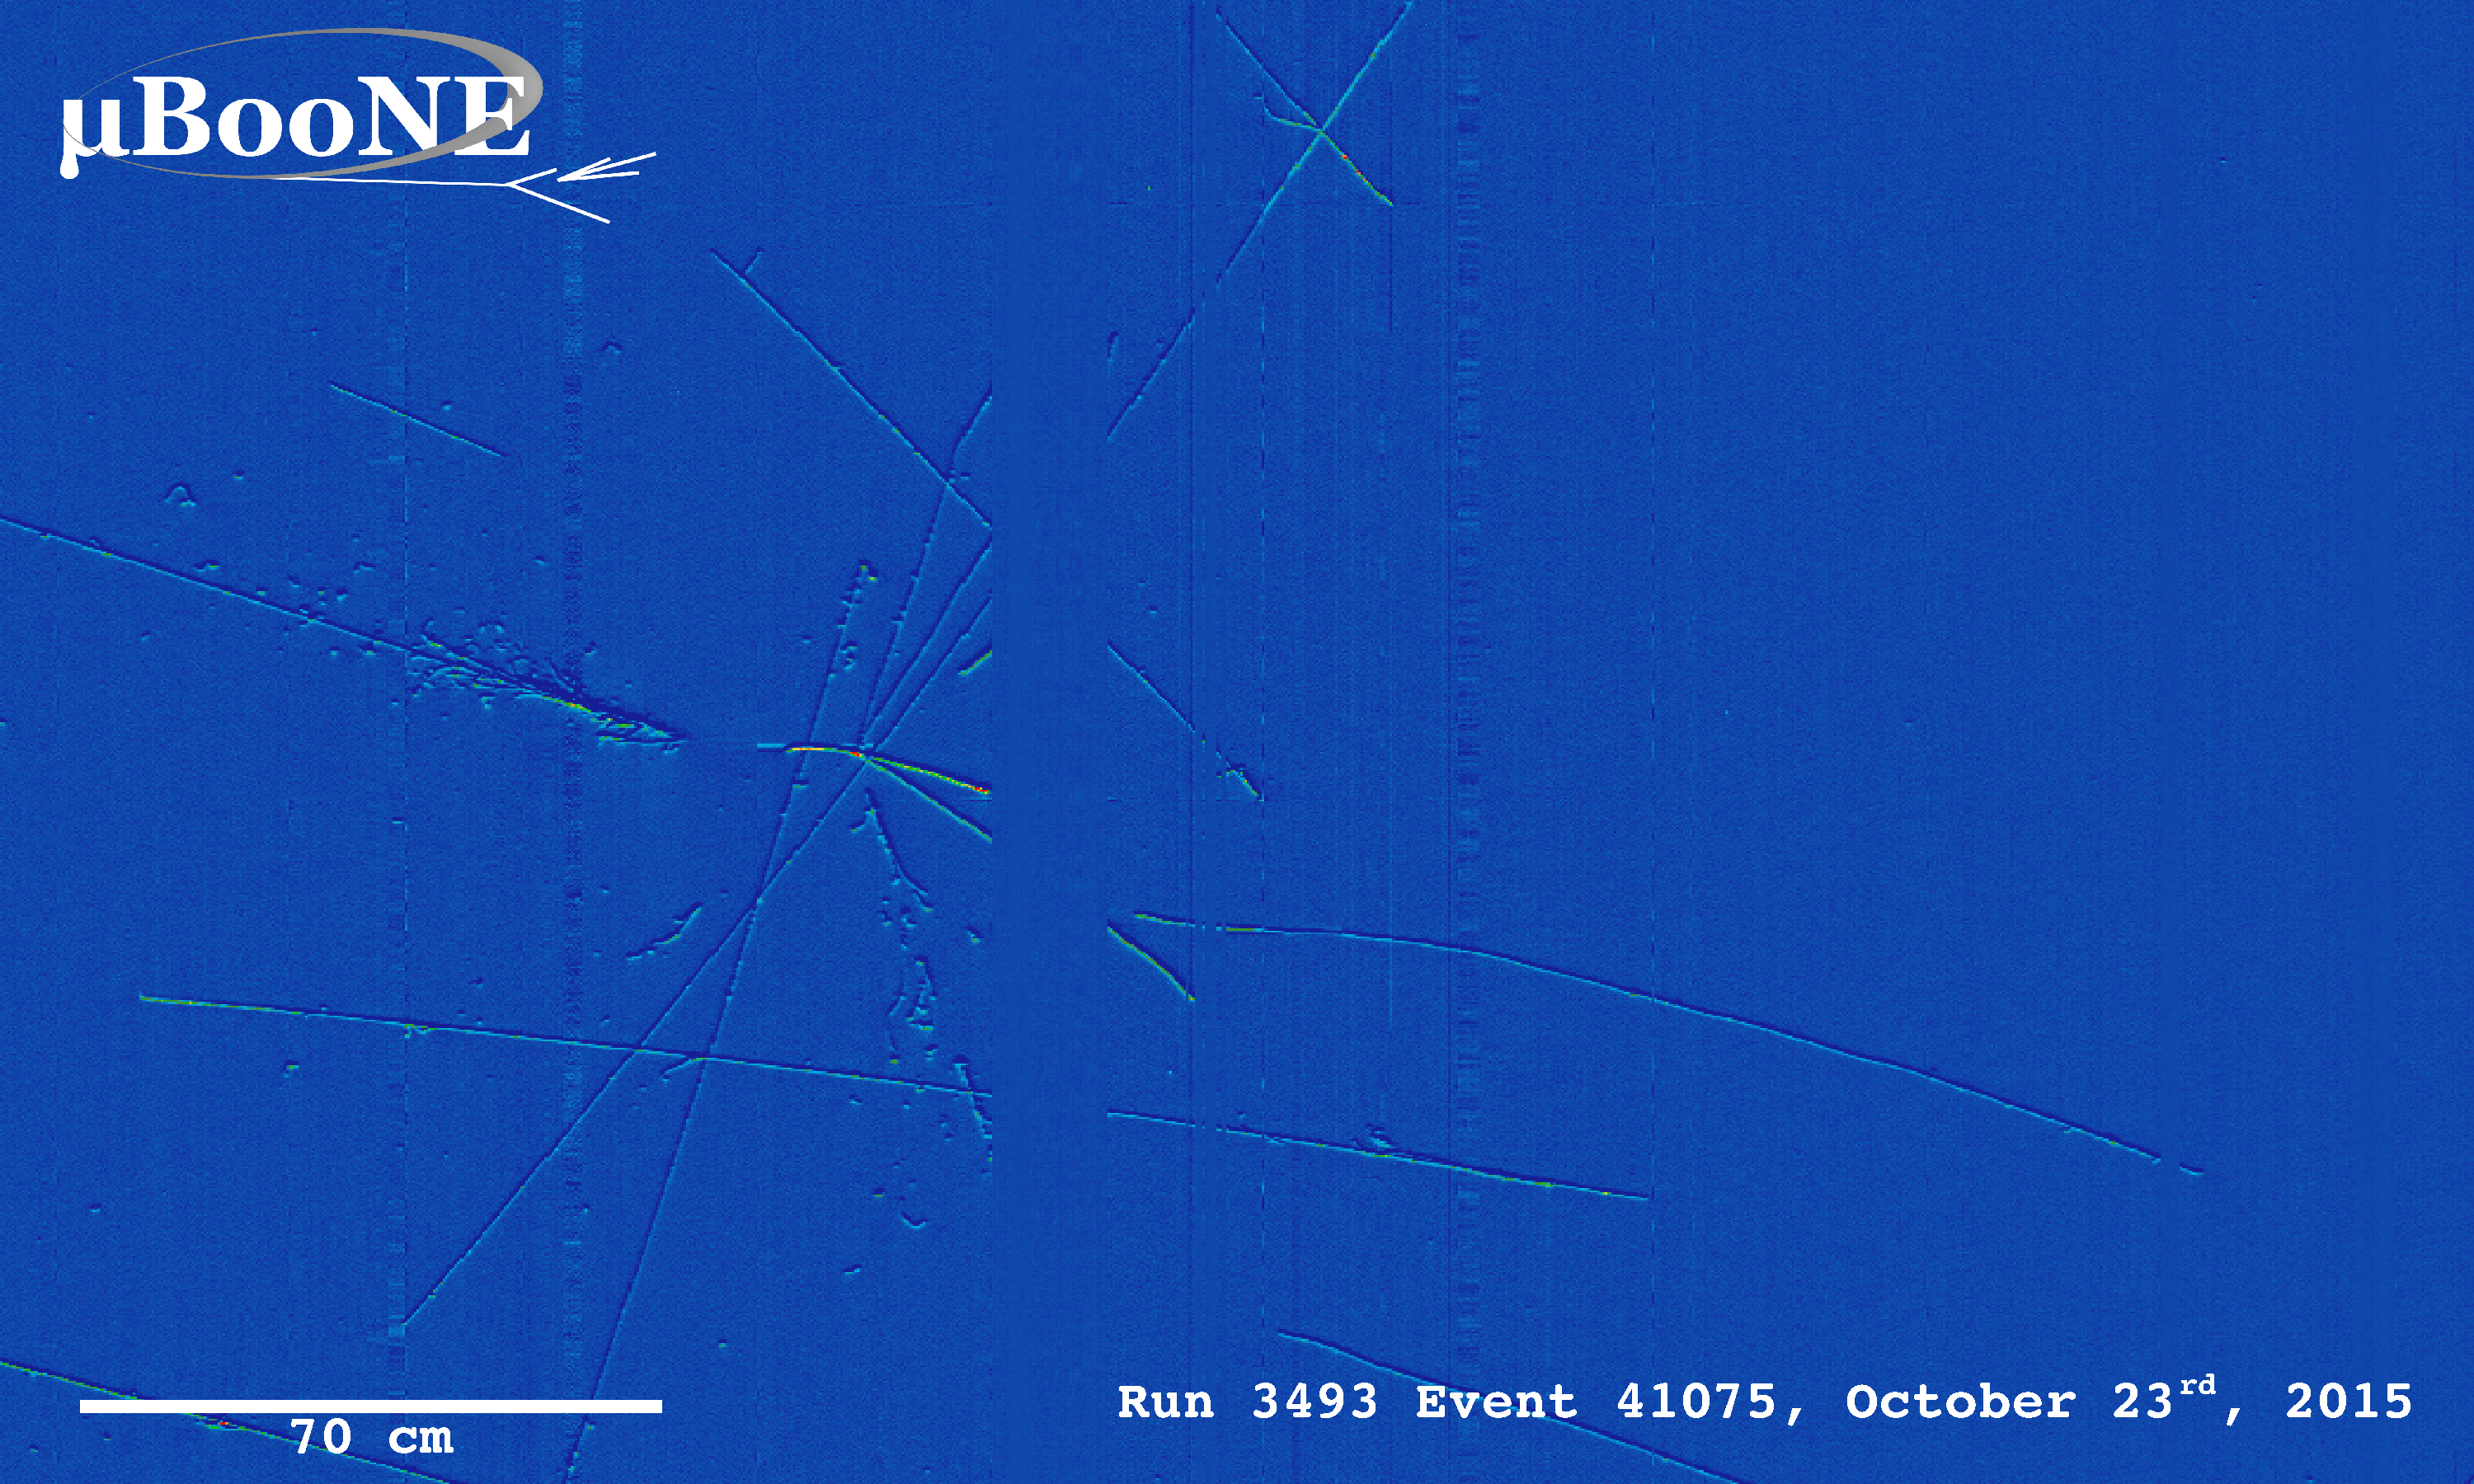
\includegraphics[width=\textwidth]{figs/first_neutrino_pdfs/run3493_subrun821_event41075_ind1.pdf}
	\end{subfigure}
	\quad
\caption{First Neutrino Interaction Candidate Events from MicroBooNE}
\label{fig:3dimage}
\end{figure}
